\documentclass[12pt,a4paper]{article}
\usepackage[spanish]{babel}
\usepackage[utf8]{inputenc}
\usepackage[T1]{fontenc}
\usepackage{lmodern}
\usepackage[table]{xcolor}
\usepackage{geometry}
\usepackage{setspace}
\usepackage{longtable}
\usepackage{booktabs}
\usepackage{array}
\usepackage{tabularx}
\usepackage{hyperref}
\usepackage{enumitem}
\usepackage{graphicx}

\geometry{margin=2.4cm}
\setstretch{1.12}
\setlength{\parindent}{0pt}
\setlength{\parskip}{0.55em}
\hypersetup{colorlinks=true, linkcolor=black, urlcolor=blue, citecolor=black}

\definecolor{PrimaryBlue}{HTML}{16324F}
\definecolor{SoftGray}{HTML}{F3F6F8}

\title{\Huge\textbf{Casos de Uso (Detallado)}\\[0.3em]\Large Plataforma Web de Mascotas 3D}
\author{Bryan Quispe}
\date{10 de mayo de 2026}

\begin{document}

\begin{titlepage}
\centering
\vspace*{1.8cm}
{\Huge\bfseries\color{PrimaryBlue} Casos de Uso (Detallado)\\[0.35em]}
{\LARGE Descripciones extensas de flujos, excepciones y reglas de negocio\\[1.2cm]}

\begin{tabular}{p{5cm} p{8cm}}
\rowcolor{SoftGray}
\textbf{Versi\'on} & 1.1 \\
\textbf{Fecha} & 16 de junio de 2026 \\
\textbf{Autor} & Bryan Quispe \\
\textbf{Alcance} & MVP en desarrollo: Mascotas urbanas/rurales, fotos y modelos 3D editables \\
\end{tabular}

\vfill
{\large Documento para compilaci\'on en Overleaf}
\end{titlepage}

\tableofcontents
\newpage

\section{Prop\'osito y alcance}
Documento de casos de uso con trazabilidad a requisitos funcionales (RF) y reglas de negocio (RN). Un caso de uso describe la interacci\'on del usuario con el sistema para alcanzar un objetivo concreto dentro de una aplicaci\'on web en desarrollo. El producto se orienta a registrar mascotas urbanas y rurales, subir fotos reales, asociar modelos 3D locales y editar transformaciones permitidas del modelo sin perder el archivo original. Incluye precondiciones, flujo normal, flujos alternos, excepciones, reglas de negocio, datos de entrada/salida y criterios de aceptaci\'on.

\section{Convenciones}
\begin{itemize}[leftmargin=*]
    \item Identificador: CU-XX
    \item Actor principal: usuario o rol humano que inicia la interacci\'on con el sistema.
    \item Actores secundarios: otros usuarios o roles humanos involucrados.
    \item Tracing: (RF-YY) indica requisito funcional relacionado.
\end{itemize}

\newpage
\section{CU-01: Registrarse en la plataforma}
\begin{tabular}{|p{3.5cm}|p{10cm}|}
\hline
\textbf{Identificador} & CU-01 \\
\hline
\textbf{Nombre} & Registrarse en la plataforma \\
\hline
\textbf{Actor principal} & Usuario no autenticado \\
\hline
\textbf{Actores secundarios} & Sistema interno \\
\hline
\textbf{Precondiciones} & El usuario accede al formulario de registro. \\
\hline
\textbf{Requisitos relacionados} & RF-01 \\
\hline
\end{tabular}

\vspace{0.5em}
\textbf{Datos de entrada}: email, contrase\~na, confirmaci\'on contrase\~na, nombre opcional.

\textbf{Datos de salida}: respuesta REST con estado 201 y objeto usuario (sin contrase\~na) o error con mensajes de validaci\'on.

\subsection*{Flujo normal (exhaustivo)}
\begin{enumerate}[leftmargin=*]
    \item Usuario completa formulario y env\'ia datos.
    \item Frontend valida formato b\'asico (email, longitud contrase\~na) y envia petici\'on POST /api/auth/register.
    \item Backend valida reglas de negocio: email \'unico, contrase\~na cumple pol\'itica (>=8 caracteres, opcional: may\'usculas/n\'umeros).
    \item Si validaci\'on OK, backend hashea contrase\~na y crea registro en tabla users.
    \item Backend retorna 201 Created con id y email.
    \item Frontend muestra mensaje de \'exito y redirige a login.
\end{enumerate}

\subsection*{Flujos alternos y excepciones}
\begin{itemize}[leftmargin=*]
    \item FA-01: Email ya registrado. Backend responde 409 Conflict con mensaje "Email ya existe". Fin del caso, se sugiere recuperar contrase\~na o usar otro email.
    \item FA-02: Contrase\~na no cumple pol\'itica. Backend responde 400 Bad Request con detalle de validaci\'on.
    \item FA-03: Error en BD (p.ej. timeouts). Backend responde 500 Internal Server Error; frontend muestra mensaje gen\'erico y permite reintento.
\end{itemize}

\subsection*{Reglas de negocio}
\begin{itemize}[leftmargin=*]
    \item RB-01: Email debe ser \'unico en la tabla users.
    \item RB-02: Contrase\~na solicitada no debe almacenarse en texto plano.
\end{itemize}

\subsection*{Criterios de aceptaci\'on}
Respuesta 201 y nuevo registro creado; pruebas E2E que validen flujo normal y FA-01/FA-02.

\subsection*{Reglas de negocio}
\begin{itemize}[leftmargin=*]
    \item RB-01: El email no puede repetirse en otro registro.
    \item RB-02: La contrase\~na debe almacenarse solo como hash.
    \item RB-03: El sistema no debe exponer la contrase\~na en ninguna respuesta.
\end{itemize}

\begin{figure}[h]
\centering
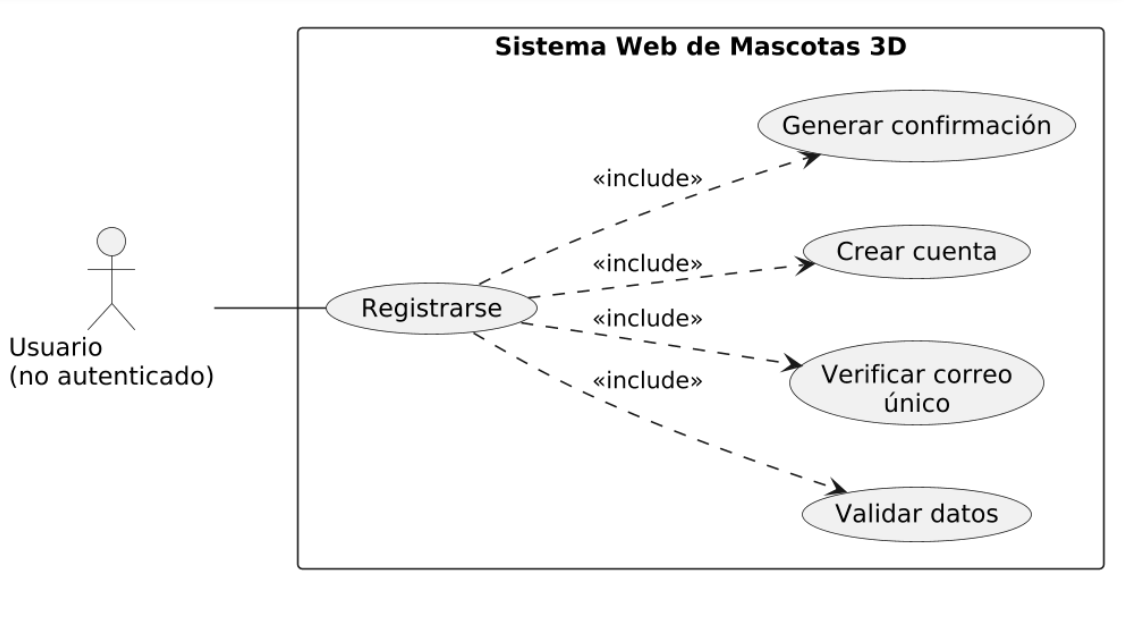
\includegraphics[width=0.82\textwidth]{diagrams/CASODEUSO1.png}
\caption{Diagrama conceptual: CU-01 Registrarse en la plataforma}
\end{figure}

\newpage
\section{CU-02: Iniciar sesi\'on}
\begin{tabular}{|p{3.5cm}|p{10cm}|}
\hline
\textbf{Identificador} & CU-02 \\
\hline
\textbf{Nombre} & Iniciar sesi\'on \\
\hline
\textbf{Actor principal} & Usuario no autenticado \\
\hline
\textbf{Actores secundarios} & Sistema interno \\
\hline
\textbf{Precondiciones} & Usuario registrado con credenciales v\'alidas. \\
\hline
\textbf{Requisitos relacionados} & RF-02 \\
\hline
\end{tabular}

\vspace{0.5em}
\textbf{Flujo normal}:
\begin{enumerate}[leftmargin=*]
    \item Usuario envia email y contrase\~na a POST /api/auth/login.
    \item Backend valida existencia de usuario y compara contrase\~na con Bcrypt.
    \item Si coincide, backend genera JWT firmado e incluye `userId` y `email` y fecha de expiraci\'on.
    \item Backend retorna 200 OK con token; frontend guarda token en almacenamiento seguro.
\end{enumerate}

\subsection*{Flujos alternos}
\begin{itemize}[leftmargin=*]
    \item FA-01: Credenciales inv\'alidas -> 401 Unauthorized con mensaje gen\'erico.
    \item FA-02: Usuario bloqueado por intentos fallidos -> 423 Locked, indicar bloqueo temporal.
\end{itemize}

\subsection*{Criterios de aceptaci\'on}
Autenticaci\'on correcta produce JWT usable para endpoints protegidos; pruebas unitarias y de integraci\'on cubren 401 y 423.

\subsection*{Reglas de negocio}
\begin{itemize}[leftmargin=*]
    \item RB-04: El token emitido debe contener identificador de usuario y expiraci\'on.
    \item RB-05: Tras varios intentos fallidos, el sistema puede bloquear temporalmente el acceso.
    \item RB-06: La sesi\'on de cliente debe caducar por inactividad seg\'un la pol\'itica del proyecto.
\end{itemize}

\begin{figure}[h]
\centering
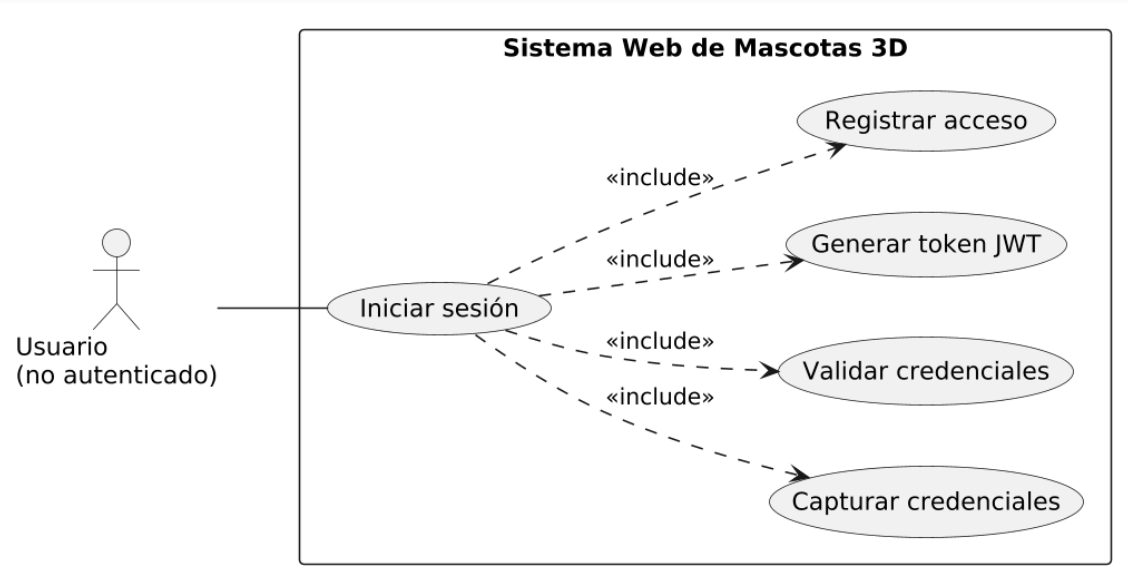
\includegraphics[width=0.82\textwidth]{diagrams/CASODEUSO2.png}
\caption{Diagrama conceptual: CU-02 Iniciar sesi\'on}
\end{figure}

\newpage
\section{CU-03: Registrar una mascota}
\begin{tabular}{|p{3.5cm}|p{10cm}|}
\hline
\textbf{Identificador} & CU-03 \\
\hline
\textbf{Nombre} & Registrar una mascota \\
\hline
\textbf{Actor principal} & Usuario autenticado \\
\hline
\textbf{Actores secundarios} & Sistema interno \\
\hline
\textbf{Precondiciones} & Token v\'alido, usuario autenticado. \\
\hline
\textbf{Requisitos relacionados} & RF-03, RF-06 (si incluye foto) \\
\hline
\end{tabular}

\vspace{0.5em}
\textbf{Flujo normal}:
\begin{enumerate}[leftmargin=*]
    \item Usuario completa formulario: nombre, edad, tipo, contexto urbano/rural y foto opcional.
    \item Usuario agrega rasgos de identificaci\'on como raza/especie, color, descripci\'on y sector referencial cuando aplique.
    \item Frontend valida campos y adjunta token en Authorization header.
    \item Backend valida token, extrae userId y valida campos obligatorios, incluido el contexto.
    \item Si hay foto, backend la procesa (comprimir/validar tipo y tama\~no) y guarda en almacenamiento.
    \item Backend crea registro en tabla mascotas con referencia al usuario, ruta de foto/modelo y clasificaci\'on urbano/rural.
    \item Backend retorna 201 con ID de mascota.
\end{enumerate}

\subsection*{Flujos alternos}
\begin{itemize}[leftmargin=*]
    \item FA-01: Token expirado -> 401 Unauthorized, frontend redirige a login.
    \item FA-02: Foto m\'as grande que 5MB -> 400 Bad Request con detalle.
    \item FA-03: Tipo de archivo no permitido -> 415 Unsupported Media Type.
\end{itemize}

\subsection*{Criterios de aceptaci\'on}
Registro creado asociado al usuario; la foto (si aplica) es accesible mediante URL segura.

\subsection*{Reglas de negocio}
\begin{itemize}[leftmargin=*]
    \item RB-07: Una mascota siempre pertenece a un solo usuario.
    \item RB-08: La foto es opcional y no debe impedir el registro b\'asico.
    \item RB-09: El sistema debe validar extensi\'on y tama\~no antes de almacenar archivos.
    \item RB-09A: Toda mascota debe clasificarse como urbana o rural para facilitar b\'usqueda y organizaci\'on.
\end{itemize}

\begin{figure}[h]
\centering
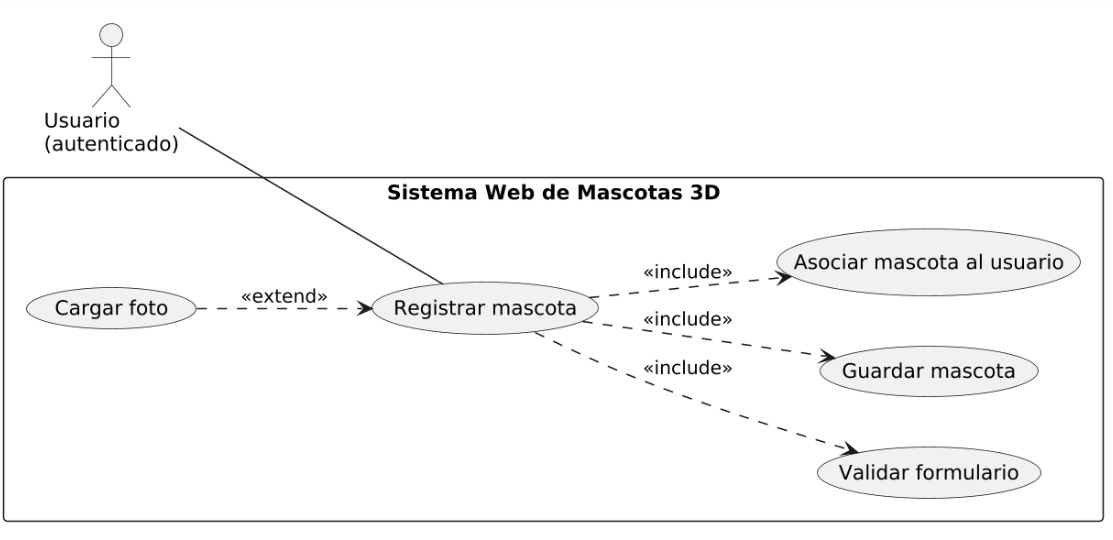
\includegraphics[width=0.82\textwidth]{diagrams/CASODEUSO3.png}
\caption{Diagrama conceptual: CU-03 Registrar una mascota}
\end{figure}

\newpage
\section{CU-04: Ver lista de mascotas}
\begin{tabular}{|p{3.5cm}|p{10cm}|}
\hline
\textbf{Identificador} & CU-04 \\
\hline
\textbf{Nombre} & Ver lista de mascotas \\
\hline
\textbf{Actor principal} & Usuario autenticado \\
\hline
\textbf{Actores secundarios} & Sistema interno \\
\hline
\textbf{Precondiciones} & Usuario autenticado con token v\'alido. \\
\hline
\textbf{Requisitos relacionados} & RF-04 \\
\hline
\end{tabular}

\vspace{0.5em}
\textbf{Flujo normal}:
\begin{enumerate}[leftmargin=*]
    \item Frontend solicita GET /api/mascotas con Authorization header.
    \item Backend valida token, consulta DB por userId, aplica paginaci\'on y filtros por contexto urbano/rural si procede.
    \item Backend retorna lista en JSON con campos: id, nombre, edad, tipo, contexto, urlFoto, fechaCreacion.
    \item Frontend renderiza la lista y permite interacci\'on (ver detalle, editar, eliminar seg\'un permisos).
\end{enumerate}

\subsection*{Flujos alternos}
\begin{itemize}[leftmargin=*]
    \item FA-01: Ninguna mascota registrada -> retornar lista vac\'ia y mostrar CTA para crear.
    \item FA-02: Error de consulta -> 500 Internal Server Error y mensaje amigable al usuario.
\end{itemize}

\subsection*{Criterios de aceptaci\'on}
La lista muestra solo mascotas del usuario; tiempos de respuesta dentro de RNF-02.

\subsection*{Reglas de negocio}
\begin{itemize}[leftmargin=*]
    \item RB-10: Solo deben mostrarse mascotas asociadas al usuario autenticado.
    \item RB-11: Si no existen registros, la vista debe mostrar un estado vac\'io expl\'icito.
    \item RB-11A: Los filtros urbano/rural no deben mezclar datos de otros usuarios.
\end{itemize}

\begin{figure}[h]
\centering
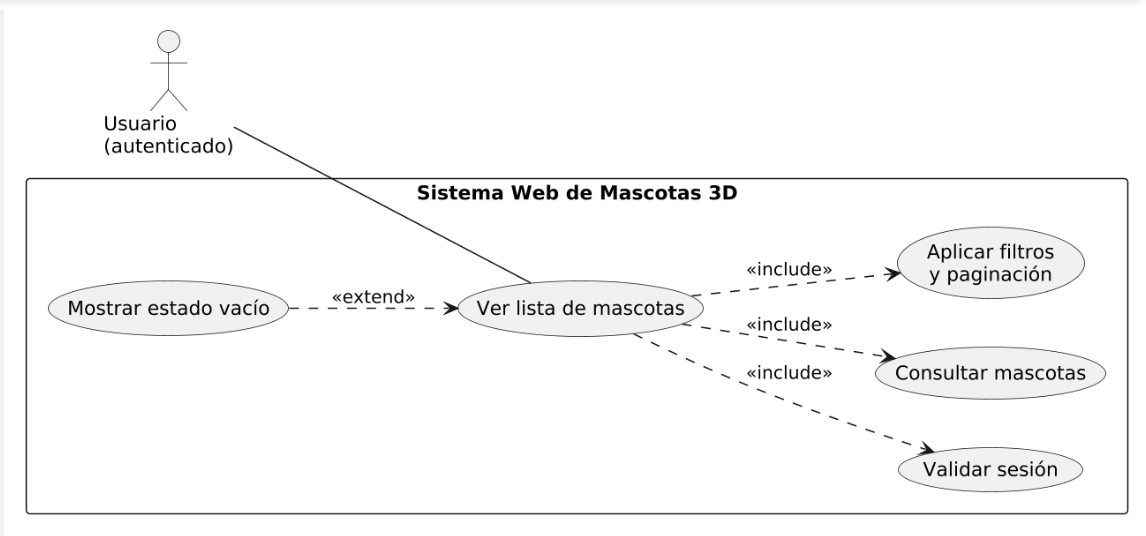
\includegraphics[width=0.82\textwidth]{diagrams/CASODEUSO4.png}
\caption{Diagrama conceptual: CU-04 Ver lista de mascotas}
\end{figure}

\newpage
\section{CU-05: Ver detalle de mascota y modelo 3D}
\begin{tabular}{|p{3.5cm}|p{10cm}|}
\hline
\textbf{Identificador} & CU-05 \\
\hline
\textbf{Nombre} & Ver detalle de mascota y modelo 3D \\
\hline
\textbf{Actor principal} & Usuario autenticado \\
\hline
\textbf{Actores secundarios} & Sistema interno \\
\hline
\textbf{Precondiciones} & Usuario autenticado y mascota existente. \\
\hline
\textbf{Requisitos relacionados} & RF-05 \\
\hline
\end{tabular}

\vspace{0.5em}
\textbf{Flujo normal}:
\begin{enumerate}[leftmargin=*]
    \item Usuario selecciona mascota en listado; frontend solicita GET /api/mascotas/{id}.
    \item Backend valida token y que la mascota pertenezca al usuario.
    \item Backend retorna detalles, fotos y la URL del modelo 3D asociado desde \texttt{backend/Modelos}.
    \item Frontend carga el modelo con Three.js. Para el cat\'alogo actual se considera OBJ/MTL con texturas JPG, con extensi\'on futura a GLB/GLTF.
    \item Frontend renderiza el canvas interactivo con rotaci\'on, zoom y controles de vista.
\end{enumerate}

\subsection*{Flujos alternos}
\begin{itemize}[leftmargin=*]
    \item FA-01: Mascota no encontrada o no pertenece al usuario -> 404 Not Found o 403 Forbidden.
    \item FA-02: Modelo 3D falla al cargar -> mostrar placeholder y permitir reintento.
\end{itemize}

\subsection*{Criterios de aceptaci\'on}
El modelo se carga correctamente en la mayoría de sesiones y permite interacci\'on b\'asica; tiempos dentro de RNF-02.

\subsection*{Reglas de negocio}
\begin{itemize}[leftmargin=*]
    \item RB-12: El detalle de una mascota solo debe mostrarse si pertenece al usuario autenticado.
    \item RB-13: Si el modelo 3D no est\'a disponible, la aplicaci\'on debe degradar a una vista segura sin bloquear la pantalla.
    \item RB-13A: El archivo original del modelo local no debe modificarse durante la visualizaci\'on.
\end{itemize}

\begin{figure}[h]
\centering
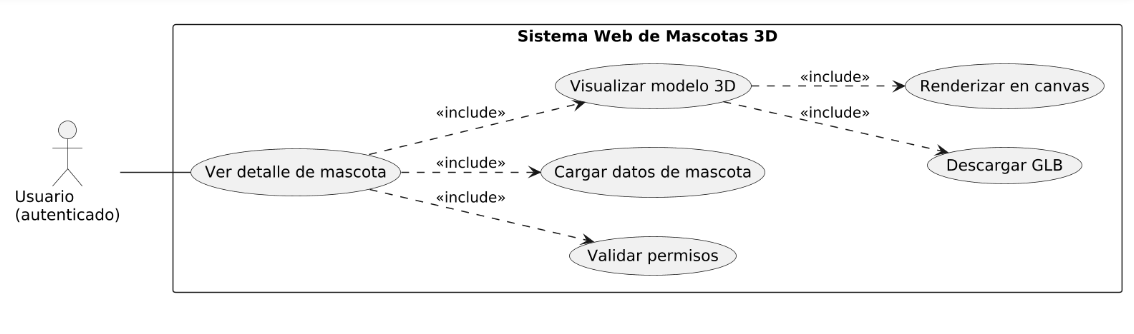
\includegraphics[width=0.82\textwidth]{diagrams/CASODEUSO5.png}
\caption{Diagrama conceptual: CU-05 Ver detalle de mascota y modelo 3D}
\end{figure}

\newpage
\section{CU-06: Expiraci\'on de sesi\'on por inactividad}
\begin{tabular}{|p{3.5cm}|p{10cm}|}
\hline
\textbf{Identificador} & CU-06 \\
\hline
\textbf{Nombre} & Expiraci\'on de sesi\'on por inactividad \\
\hline
\textbf{Actor principal} & Usuario autenticado \\
\hline
\textbf{Actores secundarios} & Sistema interno \\
\hline
\textbf{Precondiciones} & Usuario autenticado con una sesi\'on activa en el cliente. \\
\hline
\textbf{Requisitos relacionados} & RNF-05 \\
\hline
\end{tabular}

\vspace{0.5em}
\textbf{Descripci\'on}: La sesi\'on del usuario expira autom\'aticamente tras 10 minutos de inactividad o al cerrar la aplicaci\'on; no se modela como un requisito funcional independiente de logout manual.

\vspace{0.5em}
\textbf{Flujo normal}:
\begin{enumerate}[leftmargin=*]
    \item El usuario interact\'ua con la aplicaci\'on y se reinicia el contador de inactividad.
    \item El sistema monitorea el tiempo sin actividad del usuario.
    \item Cuando se alcanza el umbral de 10 minutos, el sistema invalida la sesi\'on local.
    \item El cliente elimina token y datos temporales.
    \item El usuario es redirigido a login al intentar volver a usar una ruta protegida.
\end{enumerate}

\subsection*{Criterios de aceptaci\'on}
La sesi\'on expira a los 10 minutos de inactividad y el usuario no puede seguir navegando en rutas protegidas hasta autenticarse nuevamente.

\subsection*{Flujos alternos}
\begin{itemize}[leftmargin=*]
    \item FA-01: El usuario vuelve a interactuar antes de los 10 minutos -> el temporizador se reinicia.
    \item FA-02: La aplicaci\'on se cierra -> las credenciales locales se eliminan al reiniciar la sesi\'on del cliente.
\end{itemize}

\subsection*{Reglas de negocio}
\begin{itemize}[leftmargin=*]
    \item RB-14: La expiraci\'on por inactividad debe ser autom\'atica.
    \item RB-15: El cliente no debe conservar credenciales locales despu\'es de perder la sesi\'on.
\end{itemize}

\begin{figure}[h]
\centering
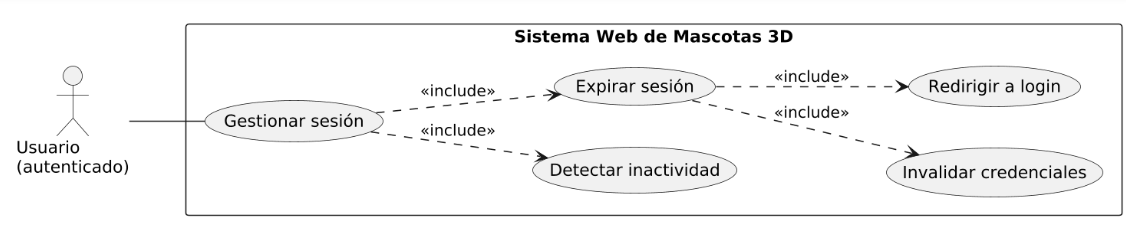
\includegraphics[width=0.82\textwidth]{diagrams/CASODEUSO6.png}
\caption{Diagrama conceptual: CU-06 Expiraci\'on de sesi\'on por inactividad}
\end{figure}

\newpage
\section{CU-07: Subir o registrar modelo 3D (Admin)}
\begin{tabular}{|p{3.5cm}|p{10cm}|}
\hline
\textbf{Identificador} & CU-07 \\
\hline
\textbf{Nombre} & Subir o registrar modelo 3D al cat\'alogo \\
\hline
\textbf{Actor principal} & Administrador (admin) \\
\hline
\textbf{Actores secundarios} & Sistema interno \\
\hline
\textbf{Precondiciones} & Admin autenticado con permisos de publicaci\'on. Los modelos locales pueden estar en \texttt{backend/Modelos}. \\
\hline
\textbf{Requisitos relacionados} & RF-07 \\
\hline
\end{tabular}

\vspace{0.5em}
\textbf{Flujo normal}:
\begin{enumerate}[leftmargin=*]
    \item Admin sube o registra archivo 3D con metadatos (nombre, tipo, contexto recomendado, versi\'on).
    \item Backend valida formato y tama\~no. En el MVP se soporta OBJ/MTL con texturas JPG y se prepara compatibilidad futura GLB/GLTF.
    \item Backend guarda o referencia archivo en almacenamiento local \texttt{backend/Modelos} y registra metadatos en DB.
    \item Backend crea versi\'on y marca el modelo como `publicado` si corresponde.
    \item Backend retorna 201 Created con id del modelo.
\end{enumerate}

\subsection*{Flujos alternativos}
\begin{itemize}[leftmargin=*]
    \item FA-01: Formato inv\'alido -> 415 Unsupported Media Type.
    \item FA-02: Tama\~no excede l\'imite -> 400 Bad Request.
    \item FA-03: Error de almacenamiento -> 500 Internal Server Error.
\end{itemize}

\subsection*{Reglas de negocio}
\begin{itemize}[leftmargin=*]
    \item RB-16: Solo el administrador puede publicar modelos 3D nuevos.
    \item RB-17: Cada subida v\'alida debe generar una versi\'on identificable.
    \item RB-18: El sistema debe conservar metadatos asociados al archivo.
    \item RB-18A: El cat\'alogo local debe conservar el modelo original sin sobrescritura por ediciones de usuario.
\end{itemize}

\subsection*{Postcondiciones}
\begin{itemize}[leftmargin=*]
    \item Modelo disponible en cat\'alogo con versi\'on asociada.
\end{itemize}

\subsection*{Criterios de aceptaci\'on}
201 Created y modelo accesible v\'ia URL; metadatos correctos.

\begin{figure}[h]
\centering
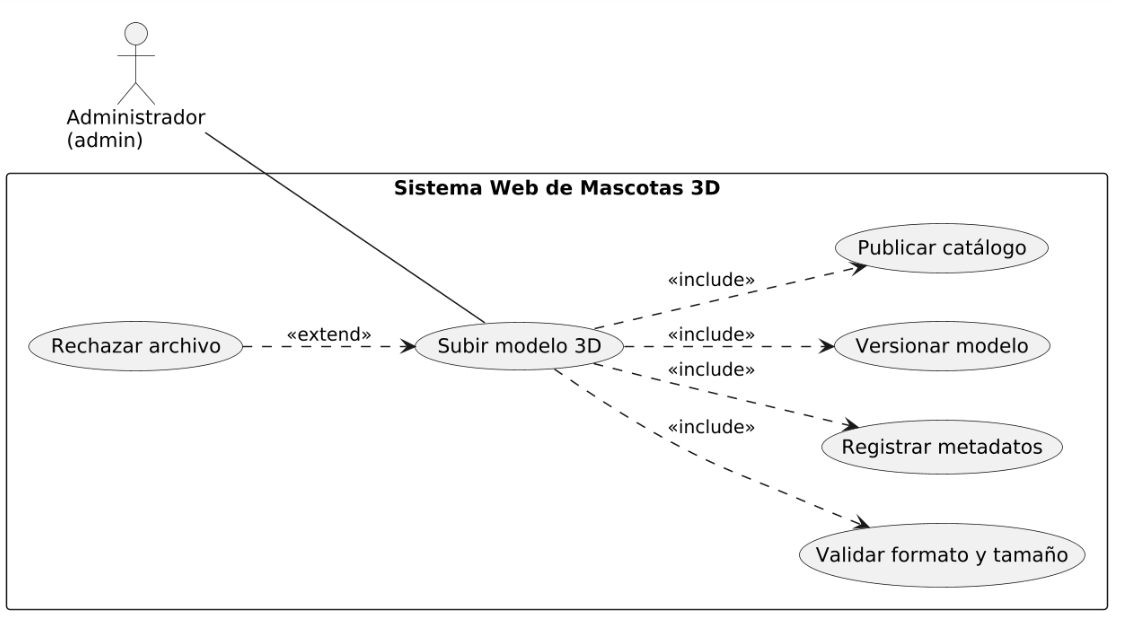
\includegraphics[width=0.82\textwidth]{diagrams/CASODEUSO7.png}
\caption{Diagrama conceptual: CU-07 Subir modelo 3D}
\end{figure}

\newpage
\section{CU-08: Editar modelo 3D de mascota (Usuario)}
\begin{tabular}{|p{3.5cm}|p{10cm}|}
\hline
\textbf{Identificador} & CU-08 \\
\hline
\textbf{Nombre} & Editar / personalizar modelo 3D de mascota \\
\hline
\textbf{Actor principal} & Usuario autenticado \\
\hline
\textbf{Actores secundarios} & Administrador \\
\hline
\textbf{Precondiciones} & Usuario autenticado; modelo disponible en \texttt{backend/Modelos} y con campos editables permitidos. \\
\hline
\textbf{Requisitos relacionados} & RF-07 \\
\hline
\end{tabular}

\vspace{0.5em}
\textbf{Flujo normal}:
\begin{enumerate}[leftmargin=*]
    \item El usuario selecciona la mascota y abre su visor 3D.
    \item El sistema carga el modelo local asociado, por ejemplo Australian Cattle Dog en OBJ/MTL con texturas JPG.
    \item El sistema valida permisos y determina qu\'e transformaciones pueden editarse.
    \item El usuario modifica escala, rotaci\'on, posici\'on, color/metadatos o nombre visible.
    \item El sistema previsualiza los cambios en tiempo real.
    \item El sistema guarda los cambios como versi\'on o transformaciones asociadas a la mascota, sin sobrescribir el archivo original.
    \item Si el cambio requiere aprobaci\'on, el sistema env\'ia la solicitud al administrador.
\end{enumerate}

\subsection*{Flujos alternativos}
\begin{itemize}[leftmargin=*]
    \item FA-01: Usuario no tiene permisos -> 403 Forbidden.
    \item FA-02: El modelo no permite edici\'on -> mostrar mensaje informativo y bloquear el formulario.
    \item FA-03: La modificaci\'on requiere aprobaci\'on -> estado `pendiente` hasta revisi\'on del admin.
\end{itemize}

\subsection*{Reglas de negocio}
\begin{itemize}[leftmargin=*]
    \item RB-19: Las ediciones deben registrar qu\'e cambi\'o y cu\'ando.
    \item RB-20: Solo se permiten campos editables definidos por el sistema.
    \item RB-21: Un cambio sensible puede requerir aprobaci\'on del administrador.
    \item RB-22: Las transformaciones del usuario se guardan separadas del archivo original del cat\'alogo.
\end{itemize}

\subsection*{Postcondiciones}
\begin{itemize}[leftmargin=*]
    \item Transformaciones actualizadas o solicitud de revisi\'on registrada.
\end{itemize}

\subsection*{Criterios de aceptaci\'on}
Transformaciones actualizadas correctamente o solicitud registrada para revisi\'on por admin.

\begin{figure}[h]
\centering
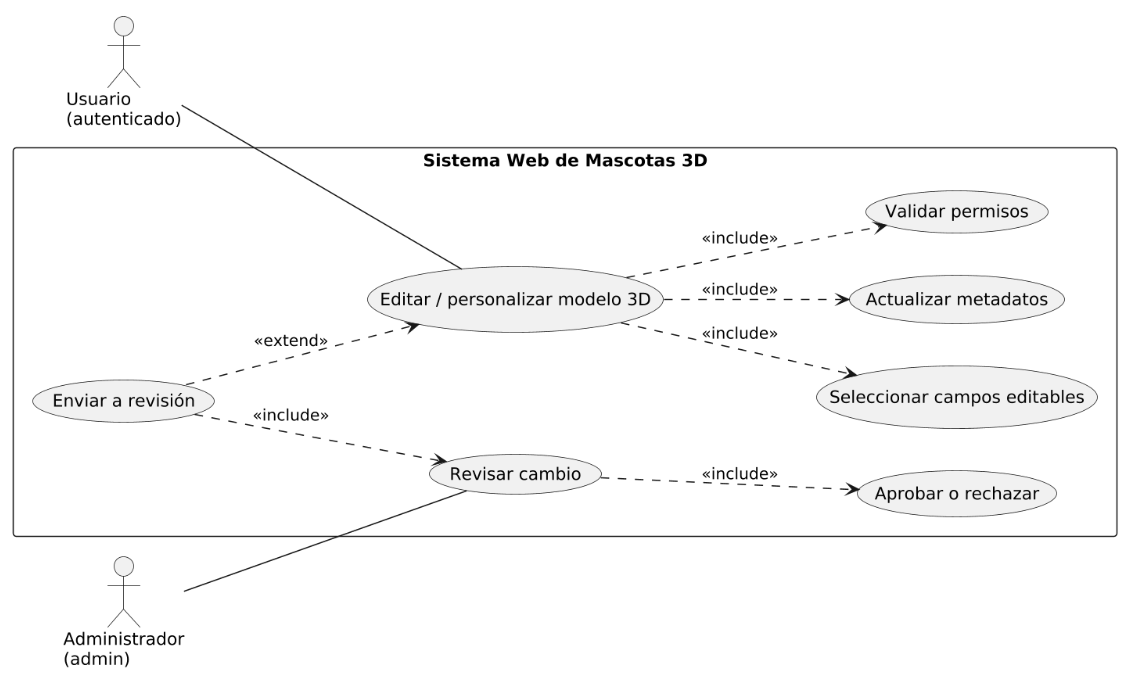
\includegraphics[width=0.82\textwidth]{diagrams/CASODEUSO8.png}
\caption{Diagrama conceptual: CU-08 Editar / personalizar modelo 3D}
\end{figure}

\newpage
\section{Anexos}
\subsection*{Matriz de trazabilidad (ejemplo)}
\begin{tabularx}{\textwidth}{l X}
\toprule
Requisito & Casos de uso relacionados \\
\midrule
RF-01 & CU-01 \\
RF-03 & CU-03 \\
RNF-05 & CU-06 \\
RF-07 & CU-07, CU-08 \\
\bottomrule
\end{tabularx}

\subsection*{Notas de implementaci\'on}
Las APIs deben devolver c\'odigos HTTP apropiados y mensajes consistentes para facilitar validaciones en frontend y pruebas autom\'aticas.

\newpage
\section{Referencias}
Fuentes y plantillas consultadas para el formato y convenciones de casos de uso:
\begin{thebibliography}{9}
\bibitem{scrumguide}
K. Schwaber y J. Sutherland,
\textit{The Scrum Guide: The Definitive Guide to Scrum: The Rules of the Game},
The Scrum Guide, 2020. Dispon\'ible en: \url{https://scrumguides.org}

\bibitem{ieee830}
IEEE,
\textit{IEEE Recommended Practice for Software Requirements Specifications},
IEEE Std 830-1998.

\bibitem{cockburn}
Alistair Cockburn,
\textit{Writing Effective Use Cases}, Addison-Wesley, 2000. (Referencia para estructura y diagramaci\'on de casos de uso)
\end{thebibliography}

\end{document}
